
%(BEGIN_QUESTION)
% Copyright 2012, Tony R. Kuphaldt, released under the Creative Commons Attribution License (v 1.0)
% This means you may do almost anything with this work of mine, so long as you give me proper credit

A Programmable Logic Controller (PLC) serves as the logic solver (safety shutdown controller) for a large motor-driven pump.  It is programmed to shut off the pump if {\it any} of the following conditions occur:

\begin{itemize}
\item{} ``Stop'' pushbutton is pressed
\item{} Pump vibrates too much
\item{} Motor becomes overloaded
\item{} Pump temperature gets too hot
\end{itemize}

$$\includegraphics[width=15.5cm]{i02115x01.eps}$$

Red LED indicator lights on the input and output cards of the PLC indicate if those respective I/O channels are energized.  The light statuses shown in the above diagram are when the pump is running as it should (i.e. no abnormal conditions).

\vskip 10pt

Suppose this pump is running just as it should.  Identify how you could electrically simulate each of the following ``trip'' conditions, causing the pump to shut down even though nothing is physically wrong with the pump:

\begin{itemize}
\item{} Electrically simulate a high-vibration condition to the PLC
\vskip 10pt
\item{} Electrically simulate an overloaded motor condition to the PLC
\vskip 10pt
\item{} Electrically simulate a high-temperature condition to the PLC
\vskip 10pt
\item{} Electrically simulate a tripped PLC (to the motor contactor)
\end{itemize}

\vskip 20pt \vbox{\hrule \hbox{\strut \vrule{} {\bf Suggestions for Socratic discussion} \vrule} \hrule}

\begin{itemize}
\item{} Identify any safety precautions to follow when working on a ``live'' 120 VAC circuit (e.g. the {\it one-hand} rule).
\end{itemize}

\underbar{file i02115}
%(END_QUESTION)





%(BEGIN_ANSWER)

\noindent
{\bf Partial answer:}

\begin{itemize}
\item{} Electrically simulate a high-temperature condition to the PLC: {\it connect a temporary jumper wire between terminal {\tt L1} and PLC input terminal {\tt X4}}
\vskip 10pt
\item{} Electrically simulate a tripped PLC (to the motor contactor): {\it open the wire connecting to PLC output terminal {\tt Y0}}
\end{itemize}


%(END_ANSWER)





%(BEGIN_NOTES)

\begin{itemize}
\item{} Electrically simulate a high-vibration condition to the PLC: {\it open the wire connecting to PLC input terminal {\tt X2}}
\vskip 10pt
\item{} Electrically simulate an overloaded motor condition to the PLC: {\it open the wire connecting to PLC input terminal {\tt X3}}
\vskip 10pt
\item{} Electrically simulate a high-temperature condition to the PLC: {\it connect a temporary jumper wire between terminal {\tt L1} and PLC input terminal {\tt X4}}
\vskip 10pt
\item{} Electrically simulate a tripped PLC (to the motor contactor): {\it open the wire connecting to PLC output terminal {\tt Y0}}
\end{itemize}




\vskip 20pt \vbox{\hrule \hbox{\strut \vrule{} {\bf Virtual Trip-testing} \vrule} \hrule}

This question is a good candidate for a ``Virtual Trip-testing'' exercise.  Presenting the diagram to students, you pose an assignment whereby students must figure out how to test some component of this system to check that it will operate as intended to shut down the system in an abnormal (trip) condition, with some realistic limitation (e.g. power cannot be shut off to the load).  Students then propose various methods for executing the test.  Your job is to determine whether or not their proposed tests will achieve the desired result(s).

During and after the exercise, it is good to ask students follow-up questions such as:

\begin{itemize}
\item{} Where might our planned test strategy go wrong?  In other words, what thing(s) might happen to foil our test, either to invalidate the results or to not honor the stated limitation(s)?
\item{} Suppose the limitation were different.  How would this affect our ability to carry out the test?
\item{} Is the last test strategy best one we could execute?
\end{itemize}



%INDEX% Safety, shutdown system: trip testing

%(END_NOTES)


